\documentclass[a4paper,12pt]{article}
%%%%%%%%%%%%%%%%%%%%%%%%%%%%%%%%%%%%%%%%%%%%%%%%%%%%%%%%%%%%%%%%%%%%%%%%%%%%%%%%%%%%%%%%%%%%%%%%%%%%%%%%%%%%%%%%%%%%%%%%%%%%%%%%%%%%%%%%%%%%%%%%%%%%%%%%%%%%%%%%%%%%%%%%%%%%%%%%%%%%%%%%%%%%%%%%%%%%%%%%%%%%%%%%%%%%%%%%%%%%%%%%%%%%%%%%%%%%%%%%%%%%%%%%%%%%
\usepackage{eurosym}
\usepackage{vmargin}
\usepackage{amsmath}
\usepackage{graphics}
\usepackage{epsfig}
\usepackage{subfigure}
\usepackage{fancyhdr}
\usepackage{listings}
\usepackage{framed}
\usepackage{graphicx}

\setcounter{MaxMatrixCols}{10}
%TCIDATA{OutputFilter=LATEX.DLL}
%TCIDATA{Version=5.00.0.2570}
%TCIDATA{<META NAME="SaveForMode" CONTENT="1">}
%TCIDATA{LastRevised=Wednesday, February 23, 2011 13:24:34}
%TCIDATA{<META NAME="GraphicsSave" CONTENT="32">}
%TCIDATA{Language=American English}

\pagestyle{fancy}
\setmarginsrb{20mm}{0mm}{20mm}{25mm}{12mm}{11mm}{0mm}{11mm}
\lhead{MA4128} \rhead{Mr. Kevin O'Brien}
\chead{Spring 2013}
%\input{tcilatex}

\begin{document}

\tableofcontents
%http://support.sas.com/publishing/pubcat/chaps/55129.pdf

\newpage
\section{Principal Component Analysis (PCA)}
\begin{itemize}
	\item Is a variable reduction technique
	\item Is used when variables are highly correlated
	\item Reduces the number of observed variables to a smaller number of principal components which account for most
	of the variance of the observed variables
	\item Is a large sample procedure
\end{itemize}

The number of components extracted is equal to the number of observed variables in the analysis. The first principal
component identified accounts for most of the variance in the data. The second component identified accounts for the
second largest amount of variance in the data and is uncorrelated with the first principal component and so on.


The total amount of variance in PCA is equal to the number of observed variables being analyzed. In PCA, observed
variables are standardized, (e.g., mean=0, standard deviation=1).

Components accounting for maximal variance are retained while other components accounting for a trivial amount of
variance are not retained. Eigenvalues indicate the amount of variance explained by each component. Eigenvectors
are the weights used to calculate components scores.


\section{High Dimensionality for Data}
\begin{itemize}
	\item Advances in data collection and storage capabilities during the past decades have led to an information
	overload in most sciences. Researchers working in domains as diverse as engineering, astronomy, biology,
	remote sensing, economics, and consumer transactions, face larger and larger observations and simulations
	on a daily basis.
	
	\item Such datasets, in contrast with smaller, more traditional datasets that have been studied
	extensively in the past, present new challenges in data analysis. 
	\item Traditional statistical methods break down
	partly because of the increase in the number of observations, but mostly because of the increase in the
	number of variables associated with each observation. The dimension of the data is the number of variables
	that are measured on each observation.
	%\\(I Fodor, LLNL, USA, June 2002).
\end{itemize}



\section{Data Reduction}
\begin{itemize}
	\item Data Reduction or Dimensionality Reduction pertains to analytic methods (typically multivariate exploratory techniques such as Factor Analysis, Multidimensional Scaling, Cluster Analysis, Canonical Correlation, or Neural Networks) that involve reducing the dimensionality of a data set by extracting a number of underlying factors, dimensions, clusters, etc., that can account for the variability in the (multidimensional) data set.
	
	\item For example, in poorly designed questionnaires, all responses provided by the participants on a large number of variables (scales, questions, or dimensions) could be explained by a very limited number of "trivial" or artifactual factors. For example, two such underlying factors could be: (1) the respondent's attitude towards the study (positive or negative) and (2) the "social desirability" factor (a response bias representing a tendency to respond in a socially desirable manner).
\end{itemize}


\subsection{Variable Redundancy}
A specific (but fictitious) example of research will now be presented to illustrate the concept of
variable redundancy introduced earlier. Imagine that you have developed a 7-item measure of
job satisfaction. The \emph{instrument} is reproduced here:


\begin{framed}
\begin{verbatim}
Please respond to each of the following statements by placing a
rating in the space to the left of the statement. In making your
ratings, use any number from 1 to 7 in which 1=�strongly disagree�
and 7=�strongly agree.�
_____ 1. My supervisor treats me with consideration.
_____ 2. My supervisor consults me concerning important decisions
that affect my work.
_____ 3. My supervisors give me recognition when I do a good job.
_____ 4. My supervisor gives me the support I need to do my job
well.
_____ 5. My pay is fair.
_____ 6. My pay is appropriate, given the amount of responsibility
that comes with my job.
_____ 7. My pay is comparable to the pay earned by other employees
whose jobs are similar to mine.
\end{verbatim}
\end{framed}

Notice that items 1-4 all deal with the same topic: the employees� satisfaction with their supervisors. In this way, items 1-4 are somewhat redundant to one another. Similarly, notice that items 5-7 also all seem to deal
with the same topic: the employees� satisfaction with their pay. Empirical findings may further support the notion that there is redundancy in the seven items. Assume that you administer the questionnaire to 200 employees and compute all possible correlations between responses to the 7 items. The resulting fictitious correlations are
reproduced in the table below.

\begin{figure}[h!]
\begin{center}
  % Requires \usepackage{graphicx}
  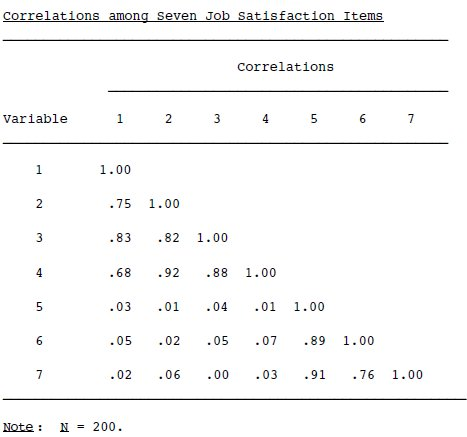
\includegraphics[scale=0.6]{3A.jpg}\\
  \caption{Questionnaire}\label{Correlations}
\end{center}

\end{figure}

When correlations among several variables are computed, they are typically summarized in the
form of a correlation matrix, such as the one reproduced in the previous table. This is an appropriate
opportunity to review just how a correlation matrix is interpreted.

The rows and columns of the table correspond to the seven variables included in the analysis: Row 1 (and column 1)
represents variable 1, row 2 (and column 2) represents variable 2, and so forth. Where a given
row and column intersect, you will find the correlation between the two corresponding variables.

\begin{itemize}
	\item For example, where the row for variable 2 intersects with the column for variable 1, you find a
	correlation of 0.75; this means that the correlation between variables 1 and 2 is 0.75.
	The correlations show that the seven items seem to hang together in two distinct
	groups.
	
\item First, notice that items 1-4 show relatively strong correlations with one another. This
	could be because items 1-4 are measuring the same construct. In the same way, items 5-7
	correlate strongly with one another (a possible indication that they all measure the same
	construct as well). 
\item Even more interesting, notice that items 1-4 demonstrate very weak
	correlations with items 5-7. This is what you would expect to see if items 1-4 and items 5-7
	were measuring two different constructs.
	
\item 	Given this apparent redundancy, it is likely that the seven items of the questionnaire are not
	really measuring seven different constructs; more likely, items 1-4 are measuring a single
	construct that could reasonably be labelled \textbf{\emph{satisfaction with supervision}} while items 5-7 are
	measuring a different construct that could be labelled \textbf{\emph{satisfaction with pay}}.
	
\item 	If responses to the seven items actually displayed the redundancy suggested by the pattern of
	correlations, it would be advantageous to somehow reduce the number of variables
	in this data set, so that (in a sense) items 1-4 are collapsed into a single new variable that reflects
	the employees� satisfaction with supervision, and items 5-7 are collapsed into a single new
	variable that reflects satisfaction with pay.
	
\item 	We could then use these two new artificial variables (rather than the seven original variables) as predictor variables in multiple regression, or in any other type of analysis.
	
\item 	In essence, this is what is accomplished by principal component analysis: it allows you to reduce
	a set of observed variables into a smaller set of artificial variables called principal components.
	The resulting principal components may then be used in subsequent analyses.
\end{itemize}

\newpage
\subsection*{Variable Reduction Procedure}

Principal component analysis is a variable reduction procedure. It is useful when you have
obtained data on a number of variables (possibly a large number of variables), and believe that
there is some redundancy in those variables. In this case, redundancy means that some of the
variables are correlated with one another, possibly because they are measuring the same
construct. Because of this redundancy, you believe that it should be possible to reduce the
observed variables into a smaller number of principal components (artificial variables) that will
account for most of the variance in the observed variables.


\section*{Principal Component Analysis}


\subsection{PCA Terminology}
\begin{itemize}
	\item  PC loadings are correlation coefficients between the PC scores and the
	original variables.
	\item  PC loadings measure the importance of each variable in accounting for the
	variability in the PC.  It is possible to interpret the first few PCs in terms of
	'overall' effect or a 'contrast' between groups of variables based on the
	structures of PC loadings.
	\item high correlation between PC1 and a variable indicates that the variable is
	associated with the direction of the maximum amount of variation in the
	dataset.
	\item More than one variable might have a high correlation with PC1. A strong
	correlation between a variable and PC2 indicates that the variable is
	responsible for the next largest variation in the data perpendicular to PC1,
	and so on.
	\item  if a variable does not correlate to any PC, or correlates only with the last PC,
	or one before the last PC, this usually suggests that the variable has little or
	no contribution to the variation in the dataset. Therefore, PCA may often
	indicate which variables in a dataset are important and which ones may be of
	little consequence. Some of these low-performance variables might
	therefore be removed from consideration in order to simplify the overall
	analyses.
\end{itemize}

\subsection*{Characteristics of Principal Components}
The first component extracted in a principal
component analysis accounts for a maximal amount of total variance in the observed variables.
Under typical conditions, this means that the first component will be correlated with at least
some of the observed variables. It may be correlated with many.

The second component extracted will have two important characteristics. First, this component
will account for a maximal amount of variance in the data set that was not accounted for by the
first component. Again under typical conditions, this means that the second component will be
correlated with some of the observed variables that did not display strong correlations with
component 1.

The second characteristic of the second component is that it will be uncorrelated with the first
component. Literally, if you were to compute the correlation between components 1 and 2, that
correlation would be zero.

The remaining components that are extracted in the analysis display the same two characteristics:
each component accounts for a maximal amount of variance in the observed variables that was
not accounted for by the preceding components, and is uncorrelated with all of the preceding
components. A principal component analysis proceeds in this fashion, with each new component
accounting for progressively smaller and smaller amounts of variance (this is why only the first
few components are usually retained and interpreted). When the analysis is complete, the
resulting components will display varying degrees of correlation with the observed variables, but
are completely uncorrelated with one another.


\section{Principal Component Analysis }

\subsection{Introduction}
Principal component analysis is appropriate when you have obtained measures on a number of
(possibly) correlated observed variables and wish to develop a smaller number of artificial uncorrelated variables called \textbf{principal components} that will account for most of the variance in the observed variables. The first principal component accounts for as much of the variability in the data as possible, and each succeeding component accounts for as much of the remaining variability as possible. The principal
components may then be used as predictor or criterion variables in subsequent analyses.


Traditionally, principal component analysis is performed can be performed on raw data, on the symmetric \textbf{Covariance matrix} or on the symmetric \textbf{Correlation matrix}. (The covariance matrix contains scaled sums of squares and cross products. A correlation matrix is like a covariance matrix but first the variables, i.e. the columns, have been standardized.)

If raw data is used, the procedure will create the original correlation matrix or covariance matrix, as specified by the user.  If the correlation matrix is used, the variables are standardized and the total variance will equal the number of variables used in the analysis (because each standardized variable has a variance equal to 1).  If the covariance matrix is used, the variables will remain in their original metric.  However, one must take care to use variables whose variances and scales are similar.  Unlike \textbf{factor analysis}, which analyzes the common variance, the original matrix in a principal components analysis analyzes the total variance.  Also, principal components analysis assumes that each original measure is collected without measurement error.





\subsection{Mathematical background of PCA}
\begin{itemize}
	\item Principal Component Analysis is a linear \textbf{dimensionality reduction} technique, which identifies orthogonal directions of maximum variance in the original data, and projects the data into a lower-dimensionality space formed of a sub-set of the highest-variance components (Bishop, 1995).
	
	
\item 	The mathematical technique used in PCA is called \textbf{eigen analysis}. Technically, a principal component can be
	defined as a linear combination of optimally-weighted observed variables.
\item  Software packages compute solutions for these weights by using a special
	type of equation called an \textbf{\emph{eigenequation}}. The weights produced by these eigenequations are
	optimal weights in the sense that, for a given set of data, no other set of weights could produce a
	set of components that are more successful in accounting for variance in the observed variables.
\item 	The weights are created so as to satisfy a principle of least squares that is similar (but not identical) to
	the principle of least squares used in multiple regression.
\end{itemize}


Remarks
\begin{itemize}
\item The words \textbf{\emph{linear combination}} refer to the fact that scores on a
component are created by adding together scores on the observed variables being analyzed.
\item \textbf{\emph{Optimally weighted}} refers to the fact that the observed variables are weighted in such a way
that the resulting components account for a maximal amount of variance in the data set.
\end{itemize}

%We solve for the eigenvalues and eigenvectors of a square symmetric matrix with sums of squares and cross products. The eigenvector associated with the largest eigenvalue has the same direction as the first principal component. Similarly the eigenvector associated with the second largest eigenvalue determines the direction of the second principal component, and so on. The sum of the eigenvalues equals the \textbf{trace} of the square matrix and the maximum number of eigenvectors equals the number of rows (or columns) of this matrix.




\subsection{Sampling adequacy (KMO Statistic)}
Measured by the Kaiser-Meyer-Olkin (KMO) statistics, sampling adequacy predicts if the analyses are likely to perform well, based on correlation and partial correlation. KMO can also be used to assess which variables to drop from the model because they are too multi-collinear.

There is a KMO statistic for each individual variable, and their sum is the KMO overall statistic. KMO varies from 0 to 1.0 and KMO overall should be 0.60 or higher to proceed with factor analysis. Values below 0.5 imply that factor analysis or PCA may not be appropriate. (Approach to overcoming this: If it is not, drop the \textbf{indicator variables} with the lowest individual KMO statistic values, until KMO overall rises above 0.60.)

Kaiser-Meyer-OlkinTo compute KMO overall, the numerator is the sum of squared correlations of all variables in the analysis (except the 1.0 self-correlations of variables with themselves, of course). The denominator is this same sum plus the sum of squared partial correlations of each variable i with each variable j, controlling for others in the analysis. The concept is that the partial correlations should not be very large if one is to expect distinct factors to emerge from factor analysis.

\subsection{Bartlett's Test for Sphericity}
Bartlett's measure tests the null hypothesis that the original correlation matrix is an identity
matrix. For PCA and factor analysis to work we need some relationships between variables and if the R-
matrix were an identity matrix then all correlation coefficients would be zero. Therefore, we
want this test to be signifcant (i.e. have a significance value less than 0.05). A significant test
tells us that the correlation matrix is not an identity matrix; therefore, there are some relationships
between the variables we hope to include in the analysis. For these data, Bartlett's test is
highly significant (p < 0.001), and therefore factor analysis is appropriate.
%====================================================%
\newpage

\section{Review of Important Definitions}
\begin{itemize}
\item An observed variable can be measured directly, is sometimes called a measured variable or an indicator or a
manifest variable.
\item A principal component is a linear combination of weighted observed variables. Principal components are
uncorrelated and orthogonal.
\item A latent construct can be measured indirectly by determining its influence to responses on measured variables. A latent construct could is also referred to as a factor, underlying construct, or unobserved variable.
\item Factor scores are estimates of underlying latent constructs.
\item Unique factors refer to unreliability due to measurement error and variation in the data.
\item Principal component analysis minimizes the sum of the squared perpendicular distances to the axis of the
principal component while least squares regression minimizes the sum of the squared distances perpendicular to the
x axis (not perpendicular to the fitted line).
\item Principal component scores are actual scores.
\item Eigenvectors are the weights in a linear transformation when computing principal component scores.
Eigenvalues indicate the amount of variance explained by each principal component or each factor.
\item Orthogonal means at a 90 degree angle, perpendicular.
Obilque means other than a 90 degree angle.
\item An observed variable \textbf{\emph{loads}} on a factors if it is highly correlated with the factor, has an eigenvector of greater magnitude on that factor.
\item Communality is the variance in observed variables accounted for by a common factors. Communality is more
relevant to EFA than PCA.
\end{itemize}
\end{document}
%--------------------------------------------------------------------------------------------------%
\section{Exploratory Factor Analysis}
Principal Component Analysis (PCA) and Exploratory Factor Analysis (EFA) are both variable reduction techniques
and sometimes mistaken as the same statistical method. However, there are distinct differences between PCA and
EFA. Similarities and differences between PCA and EFA will be examined.



\subsection{Factor Analysis}
Factor analysis is a statistical procedure to identify interrelationships that
exist among a large number of variables, i.e.,  to identify how suites of
variables are related.

Factor analysis can be used for exploratory or confirmatory purposes.
As an exploratory procedure, factor analysis is used to search for a
possible underlying structure in the variables. In confirmatory research,
the researcher evaluates how similar the actual structure of the data, as
indicated by factor analysis, is to the expected structure.

The major difference between exploratory and confirmatory factor
analysis is that researcher has formulated hypotheses about the
underlying structure of the variables when using factor analysis for
confirmatory purposes.

As an exploratory tool, factor analysis doesn't have many statistical
assumptions. The only real assumption is presence of relatedness
between the variables as represented by the correlation coefficient. If
there are no correlations, then there is no underlying structure.

\subsection{Exploratory Factor Analysis (EFA)}
\begin{itemize}
\item Is a variable reduction technique which identifies the number of \textbf{\emph{latent constructs}} and the underlying factor
structure of a set of variables
\item Hypothesizes an underlying construct, a variable not measured directly
\item Estimates factors which influence responses on observed variables
\item Allows you to describe and identify the number of latent constructs (also known as factors)
\item Includes unique factors, error due to unreliability in measurement
\item Traditionally has been used to explore the possible underlying factor structure of a set of measured variables without imposing any preconceived structure on the outcome.
\end{itemize}

The figure below shows four \textbf{\emph{factors}} (ovals) each measured by 3 observed variables (rectangles) with unique factors. Since measurement is not perfect, error or unreliability is estimated and specified explicitly in the diagram.

\textbf{\emph{Factor loadings}} (parameter estimates) help interpret factors. Loadings are the correlation between observed variables and factors, are standardized regression weights if variables are standardized (weights used to predict variables from factor). Standardized linear weights represent the effect size of the factor
on variability of observed variables.

\begin{figure}[h!]
\begin{center}
  % Requires \usepackage{graphicx}
  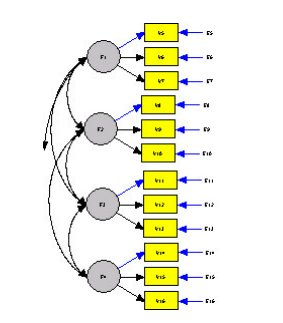
\includegraphics[scale=0.6]{4AFactor.jpg}\\
  \caption{Factor Analysis}
\end{center}
\end{figure}

In Exploratory Factor Analysis, observed variables are a linear combination of the underlying factors (estimated factor and a unique factor).

Communality is the variance of observed variables accounted for by a common factor. Large communality is strongly
influenced by an underlying construct.

\subsection{Similarities between PCA and EFA}
\begin{itemize}
\item PCA and EFA have these assumptions in common:
\begin{itemize}
\item Measurement scale is interval or ratio level
\item Random sample - at least 5 observations per observed variable and at least 100 observations.
\item Larger sample sizes recommended for more stable estimates, 10-20 observations per observed variable
\end{itemize}
\item `Over-sample' to compensate for missing values
\item Linear relationship between observed variables
\item Normal distribution for each observed variable
\item Each pair of observed variables has a bivariate normal distribution
\item PCA and EFA are both variable reduction techniques. (If communalities are large, close to 1.00, results could be similar.)
\end{itemize}

\subsection{Differences between PCA and FA}
These techniques are typically used to analyze groups of correlated variables representing one or more common domains; for example, indicators of socioeconomic status, job satisfaction, health, self-esteem, political attitudes or family values. 
Principal components analysis is used to find optimal ways of combining variables into a small number of subsets, while factor analysis may be used to identify the structure underlying such variables and to estimate scores to measure latent factors themselves. The main applications of these techniques can be found in the analysis of multiple indicators, measurement and validation of complex constructs, index and scale construction, and data reduction. These approaches are particularly useful in situations where the dimensionality of data and its structural composition are not well known.

When an investigator has a set of hypotheses that form the conceptual basis for her/his factor analysis, the investigator performs a confirmatory, or hypothesis testing, factor analysis. In contrast, when there are no guiding hypotheses, when the question is simply what are the underlying factors the investigator conducts an exploratory factor analysis. 

The factors in factor analysis are conceptualized as "real world" entities such as depression, anxiety, and disturbed thought. This is in contrast to principal components analysis (PCA), where the components are simply geometrical abstractions that may not map easily onto real world phenomena.

\subsubsection{ Treatment of Variance}

Another difference between the two approaches has to do with the variance that is analyzed. In PCA, all of the observed variance is analyzed, while in factor analysis it is only the shared variances that is analyzed.
\begin{itemize}
\item Principal Components retained account for a maximal amount of variance of observed variables.
Factors account for common variance in the data.

\item PCA Analysis decomposes correlation matrix. EFA  decomposes adjusted correlation matrix.

\item PCA: Ones on the diagonals of the correlation matrix. EFA Diagonals of correlation matrix adjusted with unique factors.

\item PCA: Minimizes sum of squared perpendicular distance to
the component axis. EFA: Estimates factors which influence responses on
observed variables.
\item PCA: Component scores are a linear combination of the
observed variables weighted by eigenvectors.
EFA: Observed variables are linear combinations of the
underlying and unique factors.
\end{itemize}


%---------------------------------------------------------------------------------------------%
\newpage


\subsection{Biplot Display of PCA}
\begin{itemize}
\item Bi-plot display is a visualization technique for investigating
the inter-relationships between the observations and
variables in multivariate data.
\item  To display a bi-plot, the data should be considered as a
matrix, in which the column represents the variable space
while the row represents the observational space.
\item  The term bi-plot means it is a plot of two dimensions with the
observation and variable spaces plotted simultaneously.
\item  In PCA, relationships between PC scores and PCA loadings
associated with any two PCs can be illustrated in a bi-plot
display
\end{itemize}


\subsection{Communality} 
Communality refers to the total amount of variance an original variable shares with all other
variables included in the analysis.This is the proportion of each variable's variance that can be explained by the principal components .  (It is denoted as $h^2$ and can be defined as the sum of squared factor loadings).

\textbf{Initial} - By definition, the initial value of the communality in a principal components analysis is 1.

\textbf{Extraction}  - The values in this column indicate the proportion of each variable's variance that can be explained by the principal components.  Variables with high values are well represented in the common factor space, while variables with low values are not well represented. They are the reproduced variances from the number of components that you have saved.  You can find these values on the diagonal of the reproduced correlation matrix.




\subsection{Exploratory Factory Analysis}



%http://support.sas.com/publishing/pubcat/chaps/55129.pdf
%-------------------------------------------------------------------------------------------------------%

\section{What Is Rotation?}
%http://jalt.org/test/PDF/Brown31.pdf
\begin{itemize}
	\item Rotation is the performing arithmetic to obtain a new set of factor loadings (similar to regression weights) from a given set.
	
	\item Rotation is any of several methods in factor analysis by which the researcher attempts to relate the calculated factors to theoretical entities. This is done differently depending upon whether the factors are believed to be correlated (oblique) or uncorrelated
	(orthogonal). 
	\item In factor analysis and principal-components analysis, rotation of the factor axes
	(dimensions) identified in the initial extraction of factors, in order to obtain simple and interpretable
	factors.
\end{itemize}

%-------------------------------------------------------------------------------------------------------%
\subsection{Introduction to Rotation}


Factor patterns and factor loadings.

After extracting the initial components, computer softwars
will create an unrotated factor pattern matrix. The rows of this matrix represent the variables
being analyzed, and the columns represent the retained components (these components would commonly be
referred to as FACTOR1, FACTOR2 and so forth in the output).

The entries in the matrix are \textbf{\emph{factor loadings}}. A factor loading is a general term for a coefficient
that appears in a factor pattern matrix or a factor structure matrix. In an analysis that results in
oblique (correlated) components, the definition for a factor loading is different depending on
whether it is in a factor pattern matrix or in a factor structure matrix.

However, the situation is simpler in an analysis that results in orthogonal components (as in the present case): In an
orthogonal analysis, factor loadings are equivalent to conventional bivariate correlations between the observed
variables and the components.
%-------------------------------------------------------------------------------------------------------%


\subsection{Varimax Rotation}
A varimax rotation is an orthogonal rotation, meaning that
it results in uncorrelated components. Compared to some other types of rotations, a varimax
rotation tends to maximize the variance of a column of the factor pattern matrix (as opposed to a
row of the matrix). This rotation is probably the most commonly used orthogonal rotation in the
social sciences.

\subsection{VARIMAX rotation in Principal Component Analysis}
%http://www.utd.edu/~herve/Abdi-rotations-pretty.pdf
\begin{itemize}
\item Varimax, which was developed by Kaiser (1958), is indubitably the most
popular rotation method by far. For varimax a simple solution means that each
factor has a small number of large loadings and a large number of zero (or small)
loadings.

\item This simplifies the interpretation because, after a varimax rotation,
each original variable tends to be associated with one (or a small number) of
factors, and each factor represents only a small number of variables. In addition,
the factors can often be interpreted from the opposition of few variables with
positive loadings to few variables with negative loadings.

%-------------------------------------------------------------------------------------------------------%

%http://data-mining-tutorials.blogspot.ie/2009/12/varimax-rotation-in-principal-component.html
\item A VARIMAX rotation is a change of coordinates used in principal component analysis (PCA) that maximizes the sum of the variances of the squared loadings. Thus, all the coefficients (squared correlation with factors) will be either large or near zero, with few intermediate values.

\item The goal is to associate each variable to at most one factor. The interpretation of the results of the PCA will be simplified. Then each variable will be associated to one and one only factor, they are split (as much as possible) into disjoint sets.
\end{itemize}


%-------------------------------------------------------------------------------------------------------%

\subsection{What is a Rotation}

Ideally, you would like to review the correlations between the variables and the
components and use this information to interpret the components; that is, to determine what
construct seems to be measured by component 1, what construct seems to be measured by
component 2, and so forth. Unfortunately, when more than one component has been retained in
an analysis, the interpretation of an unrotated factor pattern is usually quite difficult. To make
interpretation easier, you will normally perform an operation called a rotation. A rotation is a
linear transformation that is performed on the factor solution for the purpose of making the
solution easier to interpret.

%-------------------------------------------------------------------------------------------------------%

\subsection{Varimax Rotation}
A varimax rotation is an orthogonal rotation, meaning that
it results in uncorrelated components. Compared to some other types of rotations, a varimax
rotation tends to maximize the variance of a column of the factor pattern matrix (as opposed to a
row of the matrix). This rotation is probably the most commonly used orthogonal rotation in the
social sciences.

\subsection{Interpreting the Rotated Solution}

Interpreting a rotated solution means determining just what is measured by each of the retained
components. Briefly, this involves identifying the variables that demonstrate high loadings for a
given component, and determining what these variables have in common. Usually, a brief name
is assigned to each retained component that describes its content.
The first decision to be made at this stage is to decide how large a factor loading must be to be
considered ``large."

Guidelines are provided in statistical literature for testing the statistical significance of factor loadings. Given that this is an introductory treatment of principal component analysis, however, simply consider a loading
to be large if its absolute value exceeds 0.40.


\end{document}

%-------------------------------------------------------------------------------------------------------%
%\subsection{Factor loadings}
%Factor loadings refer to the Correlations between the original variables and the factors, and
%the key to understanding the underlying nature of a particular factor. Squared
%factor loadings indicate what percentage of the variance in an original variable is
%explained by a factor.
%
%
%
%Factor loadings (factor or component coefficients) : The
%factor loadings, also called component loadings in PCA, are the
%correlation coefficients between the variables (rows) and
%factors (columns).
%
%
%
%Analogous to Pearson's r, the squared factor loading is the
%percent of variance in that variable explained by the factor.
%To get the percent of variance in all the variables accounted
%for by each factor, add the sum of the squared factor
%loadings for that factor (column) and divide by the number of
%variables. (Note the number of variables equals the sum of
%their variances as the variance of a standardized variable is
%1.) This is the same as dividing the factor's eigenvalue by the
%number of variables
%http://www.ats.ucla.edu/stat/r/dae/canonical.htm
Canonical Correlation

%Item Analysis and Factor Analysis with SPSS
%http://www2.sas.com/proceedings/sugi30/203-30.pdf
\subsection{Interpreting the Rotated Solution}

Interpreting a rotated solution means determining just what is measured by each of the retained
components. Briefly, this involves identifying the variables that demonstrate high loadings for a
given component, and determining what these variables have in common. Usually, a brief name
is assigned to each retained component that describes its content.
The first decision to be made at this stage is to decide how large a factor loading must be to be
considered ``large."
Guidelines are providedd in statistical literature for testing the statistical significance of factor loadings. Given that this
is an introductory treatment of principal component analysis, however, simply consider a loading
to be ?large? if its absolute value exceeds 0.40.



%http://support.sas.com/publishing/pubcat/chaps/55129.pdf

\subsection{Creating Factor Scores or Factor-Based Scores}

Once the analysis is complete, it is often desirable to assign scores to each subject to indicate
where that subject stands on the retained components. For example, the two components
retained in the present study were interpreted as a financial giving component and an
acquaintance helping component. You may want to now assign one score to each subject to
indicate that subject?s standing on the financial giving component, and a different score to
indicate that subject?s standing on the acquaintance helping component. With this done, these
component scores could be used either as predictor variables or as criterion variables in
subsequent analyses.
Before discussing the options for assigning these scores, it is important to first draw a distinction
between factor scores versus factor-based scores. In principal component analysis, a factor
score (or component score) is a linear composite of the optimally-weighted observed variables.

Computer software can compute each subject?s factor scores for the two components
by

\begin{itemize}
	\item determining the optimal regression weights
	\item multiplying subject responses to the questionnaire items by these weights
	\item summing the products.
\end{itemize}

The resulting sum will be a given subject?s score on the component of interest. Remember that a
separate equation, with different weights, is developed for each retained component.

A factor-based score, on the other hand, is merely a linear composite of the variables that
demonstrated meaningful loadings for the component in question. For example, in the preceding
analysis, items 4, 5, and 6 demonstrated meaningful loadings for the financial giving component.

Therefore, you could calculate the factor-based score on this component for a given subject by
simply adding together his or her responses to items 4, 5, and 6. Notice that, with a factor-based
score, the observed variables are not multiplied by optimal weights before they are summed.



%-------------------------------------------------------------------------------------------------------%

http://www.floppybunny.org/robin/web/virtualclassroom/stats/statistics2/pca1.pdf
http://210.212.115.113:81/Amarnath%20Bose/RM/StudyMaterial/FactorAnalysis.pdf
http://www.ats.ucla.edu/stat/sas/library/factor_ut.htm
http://www.sagepub.com/upm-data/19710_784.pdf
http://psychweb.psy.umt.edu/denis/datadecision/factor/dd_fa_part_2_aug_2009.pdf
http://www.unt.edu/rss/class/mike/6810/Principal%20Components%20Analysis.pdf
%-------------------------------------------------------------------------------------------------------%
\subsection{Communalities}
%http://statistics.ats.ucla.edu/stat/spss/output/principal_components.htm


\subsection{Extraction Sums of Squared Loadings}

The three columns of this half of the table exactly reproduce the values given on the same row on the left side of the table.  The number of rows reproduced on the right side of the table is determined by the number of principal components whose eigenvalues are 1 or greater.

\subsection{Component Matrix} This table contains component loadings, which are the correlations between the variable and the component.  Because these are correlations, possible values range from -1 to +1.  On the /format subcommand, we used the option blank(.30), which tells SPSS not to print any of the correlations that are .3 or less.  This makes the output easier to read by removing the clutter of low correlations that are probably not meaningful anyway.

Component - The columns under this heading are the principal components that have been extracted.  As you can see by the footnote provided by SPSS (a.), two components were extracted (the two components that had an eigenvalue greater than 1).

You usually do not try to interpret the components the way that you would factors that have been extracted from a factor analysis.  Rather, most people are interested in the component scores, which are used for data reduction (as opposed to factor analysis where you are looking for underlying latent continua).  You can save the component scores to your data set for use in other analyses using the /save subcommand.
%-------------------------------------------------------------------------------------------------------%


\subsection{Other orthogonal rotations}
%http://www.utd.edu/~herve/Abdi-rotations-pretty.pdf
There are several other methods for orthogonal rotation such as the quartimax
rotation, which minimizes the number of factors needed to explain each
variable, and the equimax rotation which is a compromise between varimax
and quartimax. Other methods exist, but none approaches varimax in popularity. 

\newpage
\section{Principal Component Analysis}
PCA is defined as the orthogonal linear transformation that transforms data to a new co-ordinate system, such that the greatest variance by any projection
of the projection of the data comes to lie on the first co-ordinate (called the first principal component).

\[ Y^{T} = X^{T}W = V \Sigma \]

where $V \Sigma W^{T}$ is the singular value decomposition (SVD) of the data matrix $X^{T}$

%==========================================================================%

This is a Technique used to reduce multidimensional data sets to lower dimensions for analysis.
PCA is also known as KArhunen Loeve Transform, Hotelling Transform, and Proper Orthogonal Decomposition.

It is mostly used as tool in Exploratory Data Analysis and used for predictive models.

PCA involves calculation of Eigenvalue Deomposition/ Single Value Decomposition for a data set, usually mean centering the data for each attribute.

It is mathematically defined as an orthogonal linear transformation that transforms the data to a new co-ordinate system, such that the greatest variance
by any projection of the data comes to lie on the first co-ordinate (called the first principal component) the second greates variance ont eh second princiiapl component anf so on. 

%==========================================================================%
\newpage

\section{Overview of Course}

To ground the students in Applied Multivariate Analysis. This module serves business and mathematics students. It introduces the mathematical statistical ideas behind \begin{itemize} \item Principal Component Analysis, \item Factor Analysis, \item Cluster Analysis, \item Discrimination Function, \item The Multiple Linear Logistic function. \end{itemize}
The students learn how to implement these techniques in SPSS to become competent in the analysis of a wide variety of multivariate data structures.

\subsection{Data Reduction in Exploratory Graphics}

The term can also refer in \textbf{exploratory graphics} to ``Data Reduction by unbiased decreasing of the sample size". This type of Data Reduction is applied in exploratory graphical data analysis of extremely large data sets. The size of the data set can obscure an existing pattern (especially in large line graphs or scatterplots) due to the density of markers or lines. Then, it can be useful to plot only a representative subset of the data (so that the pattern is not hidden by the number of point markers) to reveal the otherwise obscured but still reliable pattern.


\end{document}